\documentclass[a4paper]{book}
\usepackage{a4wide}
\usepackage{makeidx}
\usepackage{fancyhdr}
\usepackage{graphicx}
\usepackage{multicol}
\usepackage{float}
\usepackage{textcomp}
\usepackage{alltt}
\usepackage[utf8]{inputenc}
\usepackage{doxygen}
\makeindex
\setcounter{tocdepth}{1}
\renewcommand{\footrulewidth}{0.4pt}
\begin{document}
\begin{titlepage}
\vspace*{7cm}
\begin{center}
{\Large FSMEmulator Reference Manual}\\
\vspace*{1cm}
{\large Generated by Doxygen 1.5.4}\\
\vspace*{0.5cm}
{\small Sat Jan 10 10:30:46 2009}\\
\end{center}
\end{titlepage}
\clearemptydoublepage
\pagenumbering{roman}
\tableofcontents
\clearemptydoublepage
\pagenumbering{arabic}
\chapter{FSMEmulator Hierarchical Index}
\section{FSMEmulator Class Hierarchy}
This inheritance list is sorted roughly, but not completely, alphabetically:\begin{CompactList}
\item \contentsline{section}{EmulApp}{\pageref{classEmulApp}}{}
\item \contentsline{section}{Log}{\pageref{classLog}}{}
\begin{CompactList}
\item \contentsline{section}{Debug}{\pageref{classDebug}}{}
\item \contentsline{section}{Error}{\pageref{classError}}{}
\item \contentsline{section}{Warning}{\pageref{classWarning}}{}
\end{CompactList}
\item \contentsline{section}{ReentrancyPreventer}{\pageref{structReentrancyPreventer}}{}
\item \contentsline{section}{SoundPlayer}{\pageref{classSoundPlayer}}{}
\item \contentsline{section}{Status}{\pageref{classStatus}}{}
\end{CompactList}

\chapter{FSMEmulator Class Index}
\section{FSMEmulator Class List}
Here are the classes, structs, unions and interfaces with brief descriptions:\begin{CompactList}
\item\contentsline{section}{{\bf Debug} (Stream-like class to print a debug message to the app's console window Example: )}{\pageref{classDebug}}{}
\item\contentsline{section}{{\bf EmulApp} (The central class to the program that more-or-less encapsulates most objects and data in the program )}{\pageref{classEmulApp}}{}
\item\contentsline{section}{{\bf Error} (Stream-like class to print an error message to the app's console window Example: )}{\pageref{classError}}{}
\item\contentsline{section}{{\bf Log} (Super class of \doxyref{Debug}{p.}{classDebug}, \doxyref{Warning}{p.}{classWarning}, \doxyref{Error}{p.}{classError} classes )}{\pageref{classLog}}{}
\item\contentsline{section}{{\bf ReentrancyPreventer} (A helper class that helps prevent reentrancy into certain functions )}{\pageref{structReentrancyPreventer}}{}
\item\contentsline{section}{{\bf SoundPlayer} }{\pageref{classSoundPlayer}}{}
\item\contentsline{section}{{\bf Status} (Stream-like class to print a message to the app's status bar )}{\pageref{classStatus}}{}
\item\contentsline{section}{{\bf Warning} (Stream-like class to print a warning message to the app's console window )}{\pageref{classWarning}}{}
\end{CompactList}

\chapter{FSMEmulator Class Documentation}
\section{Debug Class Reference}
\label{classDebug}\index{Debug@{Debug}}
Stream-like class to print a debug message to the app's console window Example:.  


{\tt \#include $<$Log.h$>$}

Inheritance diagram for Debug:\nopagebreak
\begin{figure}[H]
\begin{center}
\leavevmode
\includegraphics[width=45pt]{classDebug__inherit__graph}
\end{center}
\end{figure}
Collaboration diagram for Debug:\nopagebreak
\begin{figure}[H]
\begin{center}
\leavevmode
\includegraphics[width=45pt]{classDebug__coll__graph}
\end{center}
\end{figure}


\subsection{Detailed Description}
Stream-like class to print a debug message to the app's console window Example:. 



\begin{Code}\begin{verbatim}        Debug() << "This is a debug message"; // would print a debug message to the console window
\end{verbatim}
\end{Code}

 

Definition at line 34 of file Log.h.

The documentation for this class was generated from the following files:\begin{CompactItemize}
\item 
Log.h\item 
Log.cpp\end{CompactItemize}

\section{EmulApp Class Reference}
\label{classEmulApp}\index{EmulApp@{EmulApp}}
The central class to the program that more-or-less encapsulates most objects and data in the program.  


{\tt \#include $<$EmulApp.h$>$}

Collaboration diagram for EmulApp:\nopagebreak
\begin{figure}[H]
\begin{center}
\leavevmode
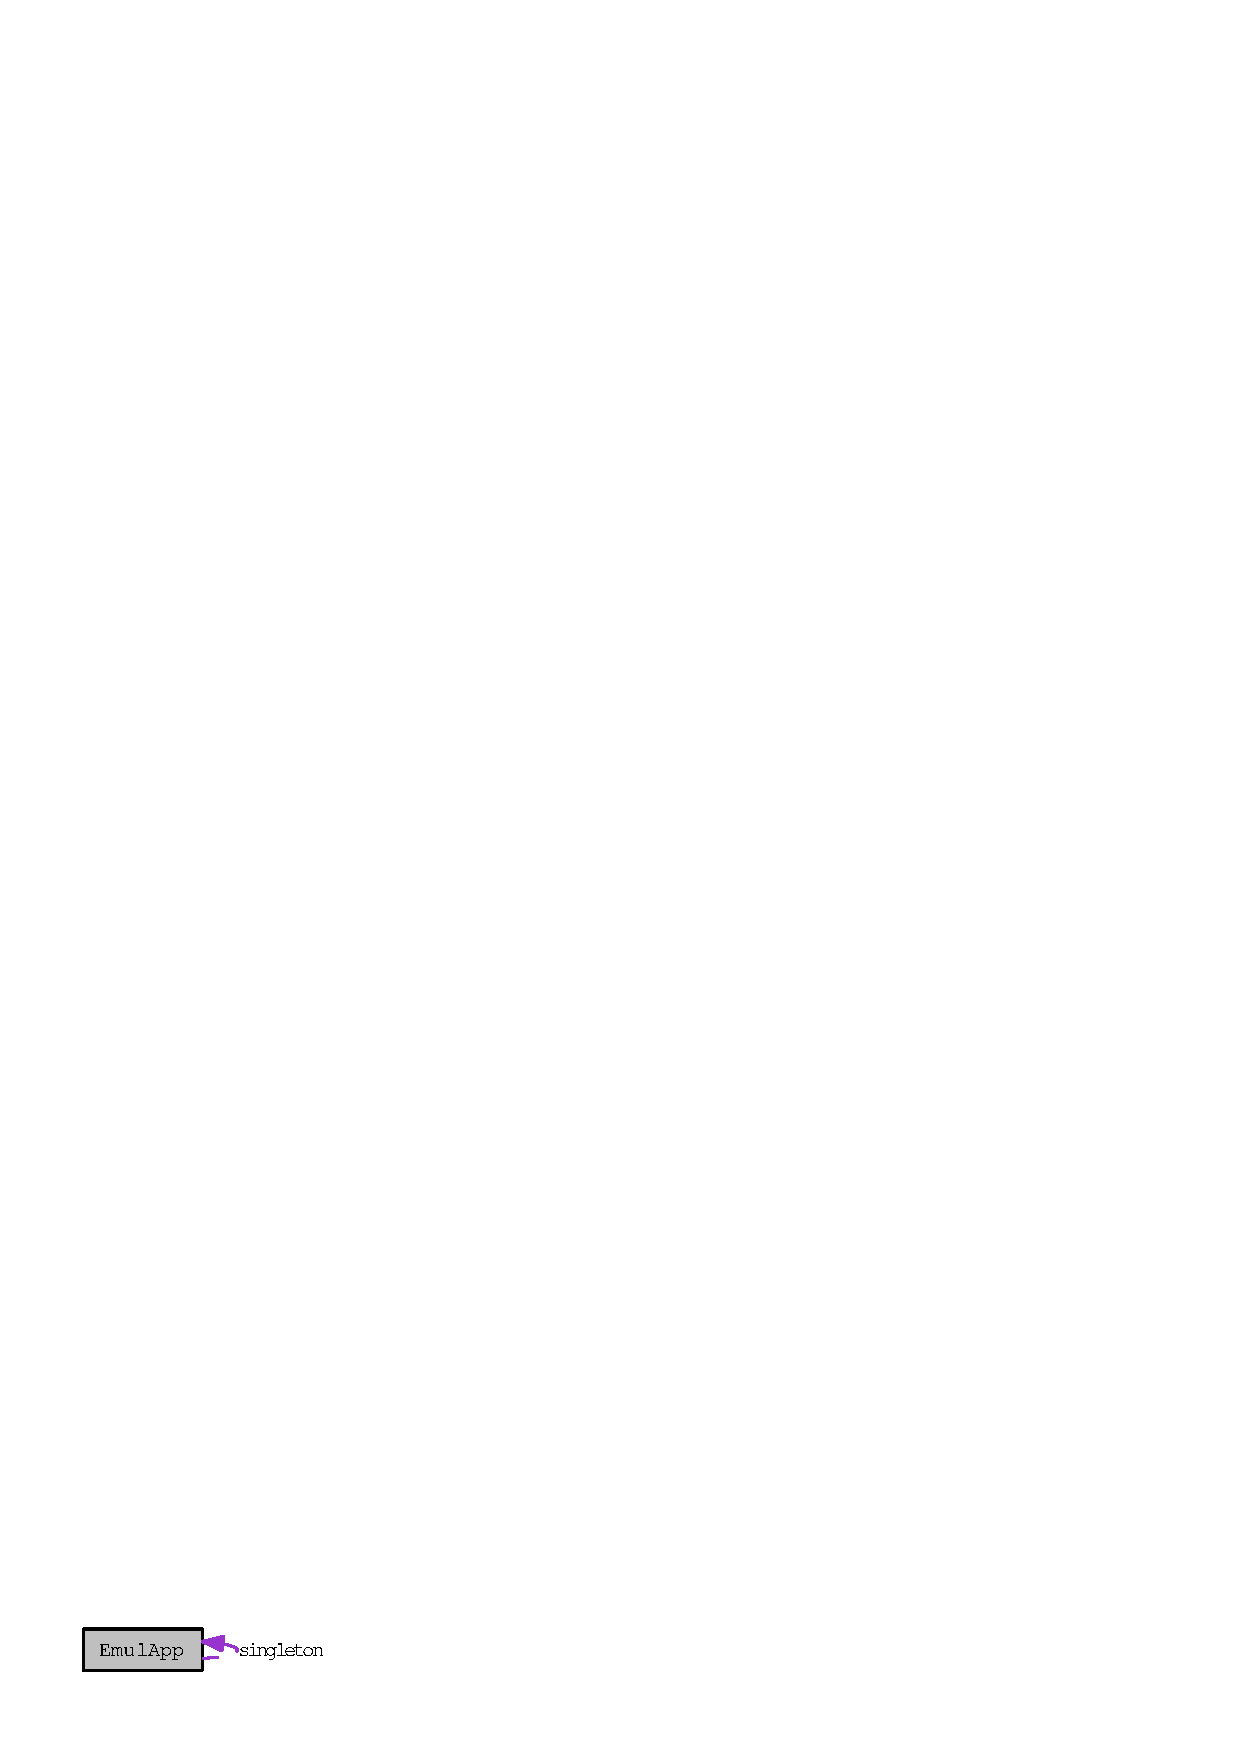
\includegraphics[width=79pt]{classEmulApp__coll__graph}
\end{center}
\end{figure}
\subsection*{Public Types}
\begin{CompactItemize}
\item 
enum {\bf EventsTypes} \{ \par
{\bf LogLineEventType} =  QEvent::User, 
{\bf StatusMsgEventType}, 
{\bf QuitEventType}, 
{\bf SoundTrigEventType}, 
\par
\textbf{SoundEventType}
 \}
\end{CompactItemize}
\subsection*{Public Slots}
\begin{CompactItemize}
\item 
void {\bf setDebugMode} (bool)\label{classEmulApp_3fa9a6ca873e638d469b2faabe0ac123}

\begin{CompactList}\small\item\em Set/unset the application-wide 'debug' mode setting. If the application is in debug mode, Debug() messages are printed to the console window, otherwise they are not. \item\end{CompactList}\item 
void \textbf{about} ()\label{classEmulApp_64daeac4b817d6c13d59cff1edcbfa2b}

\item 
void \textbf{restartFSMAndServer} ()\label{classEmulApp_621d199d1198e48ebbc2d081234eab06}

\item 
void \textbf{showProcFileViewer} ()\label{classEmulApp_7b8a405bc33d555a39d95549e5258da6}

\item 
void \textbf{showModParmsViewer} ()\label{classEmulApp_f4506b3536294818288dc4eb0d0a6504}

\item 
void \textbf{showControlWin} ()\label{classEmulApp_b9b2f6d055f5c1b8fb8d208edc1c810c}

\end{CompactItemize}
\subsection*{Public Member Functions}
\begin{CompactItemize}
\item 
MainWindow $\ast$ {\bf mainWindow} () const \label{classEmulApp_7538aa89fa904eab78f960b58f3f2f38}

\begin{CompactList}\small\item\em Returns a pointer to the application-wide ConsoleWindow instance. \item\end{CompactList}\item 
bool {\bf isDebugMode} () const \label{classEmulApp_0b6be73c5b64502d0589f8cac2d252cb}

\begin{CompactList}\small\item\em Returns true iff the application's console window has debug output printing enabled. \item\end{CompactList}\item 
void {\bf logLine} (const QString \&line, const QColor \&=QColor())
\begin{CompactList}\small\item\em Thread-safe logging -- logs a line to the log window in a thread-safe manner. \item\end{CompactList}\item 
void {\bf statusMsg} (const QString \&message, int timeout\_\-msecs=0)\label{classEmulApp_5f3359b37dfa26482034792386e65aac}

\begin{CompactList}\small\item\em Display a message to the status bar. \item\end{CompactList}\item 
bool {\bf eventFilter} (QObject $\ast$watched, QEvent $\ast$event)\label{classEmulApp_660011d09186b6ae53f4a3b52f7f954b}

\begin{CompactList}\small\item\em Used to catch various events from other threads, etc. \item\end{CompactList}\item 
bool {\bf busy} () const \label{classEmulApp_59421842f7ceb717d68eea9fb5935d16}

\begin{CompactList}\small\item\em Returns true if and only if the application is still initializing and not done with its startup. This is mainly used by the socket connection code to make incoming connections stall until the application is finished initializing. \item\end{CompactList}\end{CompactItemize}
\subsection*{Static Public Member Functions}
\begin{CompactItemize}
\item 
static {\bf EmulApp} $\ast$ {\bf instance} ()\label{classEmulApp_4e4ccc974fc75b59e57f07d85224786b}

\begin{CompactList}\small\item\em Returns a pointer to the singleton instance of this class, if one exists, otherwise returns 0. \item\end{CompactList}\end{CompactItemize}
\subsection*{Protected Slots}
\begin{CompactItemize}
\item 
void {\bf updateStatusBar} ()\label{classEmulApp_acbfa1b7996f66c9949c0662db0065c6}

\begin{CompactList}\small\item\em Called from a timer every $\sim$250 ms to update the status bar at the bottom of the console window. \item\end{CompactList}\item 
void {\bf fsmServerHasOutput} ()\label{classEmulApp_5c06a2370d22a9270285cb42b860f01d}

\begin{CompactList}\small\item\em reads all stdout from fsm server and posts it to the log \item\end{CompactList}\item 
void {\bf soundServerHasOutput} ()\label{classEmulApp_55a4c7df83e3552e074e0dca299ff604}

\begin{CompactList}\small\item\em reads all stdout from sound server and posts it to the log \item\end{CompactList}\item 
void {\bf applyModParams} ()\label{classEmulApp_8a16420a03370c1d4787d92debcfbd4d}

\begin{CompactList}\small\item\em connected to applyParamsBut clicked(), applies params, restarts fsm \item\end{CompactList}\item 
void {\bf revertModParams} ()
\begin{CompactList}\small\item\em connected to revertParamsBut clicked(), reverts params, disables buttons \item\end{CompactList}\item 
void {\bf modParamsChanged} ()\label{classEmulApp_952fdfa8fdfe3474164aa305334159a2}

\begin{CompactList}\small\item\em enables the applyParamsBut \item\end{CompactList}\item 
void \textbf{processError} (QProcess::ProcessError)\label{classEmulApp_ca6f8e9f7938de117b5c08e69a5570f7}

\item 
void \textbf{processDied} ()\label{classEmulApp_d9c86b319b6753914deefa7541f452a6}

\end{CompactItemize}
\subsection*{Protected Attributes}
\begin{CompactItemize}
\item 
volatile int {\bf lastSndEvt}\label{classEmulApp_2183269c06198dd73053d1b0bf7d5711}

\begin{CompactList}\small\item\em read/written by class SndThr and also by EmulApp::trigSound(int) \item\end{CompactList}\end{CompactItemize}
\subsection*{Friends}
\begin{CompactItemize}
\item 
class \textbf{SndThr}\label{classEmulApp_672ca163171b89dddeb7efe0e527695b}

\item 
int \textbf{main} (int, char $\ast$$\ast$)\label{classEmulApp_2c3f6775325c30275d11c6abee2db6a0}

\end{CompactItemize}
\subsection*{Classes}
\begin{CompactItemize}
\item 
struct \textbf{FSMPrintFunctor}
\end{CompactItemize}


\subsection{Detailed Description}
The central class to the program that more-or-less encapsulates most objects and data in the program. 

This class inherits from QApplication for simplicity. It is sort of a central place that other parts of the program use to find settings, pointers to other windows, and various other application-wide data. 

Definition at line 29 of file EmulApp.h.

\subsection{Member Enumeration Documentation}
\index{EmulApp@{EmulApp}!EventsTypes@{EventsTypes}}
\index{EventsTypes@{EventsTypes}!EmulApp@{EmulApp}}
\subsubsection{\setlength{\rightskip}{0pt plus 5cm}enum {\bf EmulApp::EventsTypes}}\label{classEmulApp_303c04f66d16a041b2d18e29cd4d5e2d}


\begin{Desc}
\item[Enumerator: ]\par
\begin{description}
\index{LogLineEventType@{LogLineEventType}!EmulApp@{EmulApp}}\index{EmulApp@{EmulApp}!LogLineEventType@{LogLineEventType}}\item[{\em 
LogLineEventType\label{classEmulApp_303c04f66d16a041b2d18e29cd4d5e2df88bac98a996141d8c38c8d48af1afc7}
}]used to catch log line events see \doxyref{EmulApp.cpp}{p.}{EmulApp_8cpp-source} \index{StatusMsgEventType@{StatusMsgEventType}!EmulApp@{EmulApp}}\index{EmulApp@{EmulApp}!StatusMsgEventType@{StatusMsgEventType}}\item[{\em 
StatusMsgEventType\label{classEmulApp_303c04f66d16a041b2d18e29cd4d5e2dab0b48614c5d6c36686b4e45c88786dd}
}]used to indicate the event contains a status message for the status bar \index{QuitEventType@{QuitEventType}!EmulApp@{EmulApp}}\index{EmulApp@{EmulApp}!QuitEventType@{QuitEventType}}\item[{\em 
QuitEventType\label{classEmulApp_303c04f66d16a041b2d18e29cd4d5e2dbca5931edc20aecbe14bdc2c3e4a3d79}
}]so we can post quit events.. \index{SoundTrigEventType@{SoundTrigEventType}!EmulApp@{EmulApp}}\index{EmulApp@{EmulApp}!SoundTrigEventType@{SoundTrigEventType}}\item[{\em 
SoundTrigEventType\label{classEmulApp_303c04f66d16a041b2d18e29cd4d5e2dfab573322fd03abb938b771077b72645}
}]so we can post sound trigger events... \end{description}
\end{Desc}



Definition at line 60 of file EmulApp.h.

\subsection{Member Function Documentation}
\index{EmulApp@{EmulApp}!logLine@{logLine}}
\index{logLine@{logLine}!EmulApp@{EmulApp}}
\subsubsection{\setlength{\rightskip}{0pt plus 5cm}void EmulApp::logLine (const QString \& {\em line}, const QColor \& {\em c} = {\tt QColor()})}\label{classEmulApp_eed117d40c6220478c7a58d96a93a2f7}


Thread-safe logging -- logs a line to the log window in a thread-safe manner. 

Returns the directory under which all plugin data files are to be saved. 

Definition at line 491 of file EmulApp.cpp.

Referenced by fsmServerHasOutput(), and soundServerHasOutput().\index{EmulApp@{EmulApp}!revertModParams@{revertModParams}}
\index{revertModParams@{revertModParams}!EmulApp@{EmulApp}}
\subsubsection{\setlength{\rightskip}{0pt plus 5cm}void EmulApp::revertModParams ()\hspace{0.3cm}{\tt  [protected, slot]}}\label{classEmulApp_f592f84e4877b72aa35c725bcf5ce729}


connected to revertParamsBut clicked(), reverts params, disables buttons 

connected to applyParamsBut clicked(), applies params, restarts fsm 

Definition at line 865 of file EmulApp.cpp.

The documentation for this class was generated from the following files:\begin{CompactItemize}
\item 
EmulApp.h\item 
EmulApp.cpp\end{CompactItemize}

\section{Error Class Reference}
\label{classError}\index{Error@{Error}}
Stream-like class to print an error message to the app's console window Example:.  


{\tt \#include $<$Log.h$>$}

Inheritance diagram for Error:\nopagebreak
\begin{figure}[H]
\begin{center}
\leavevmode
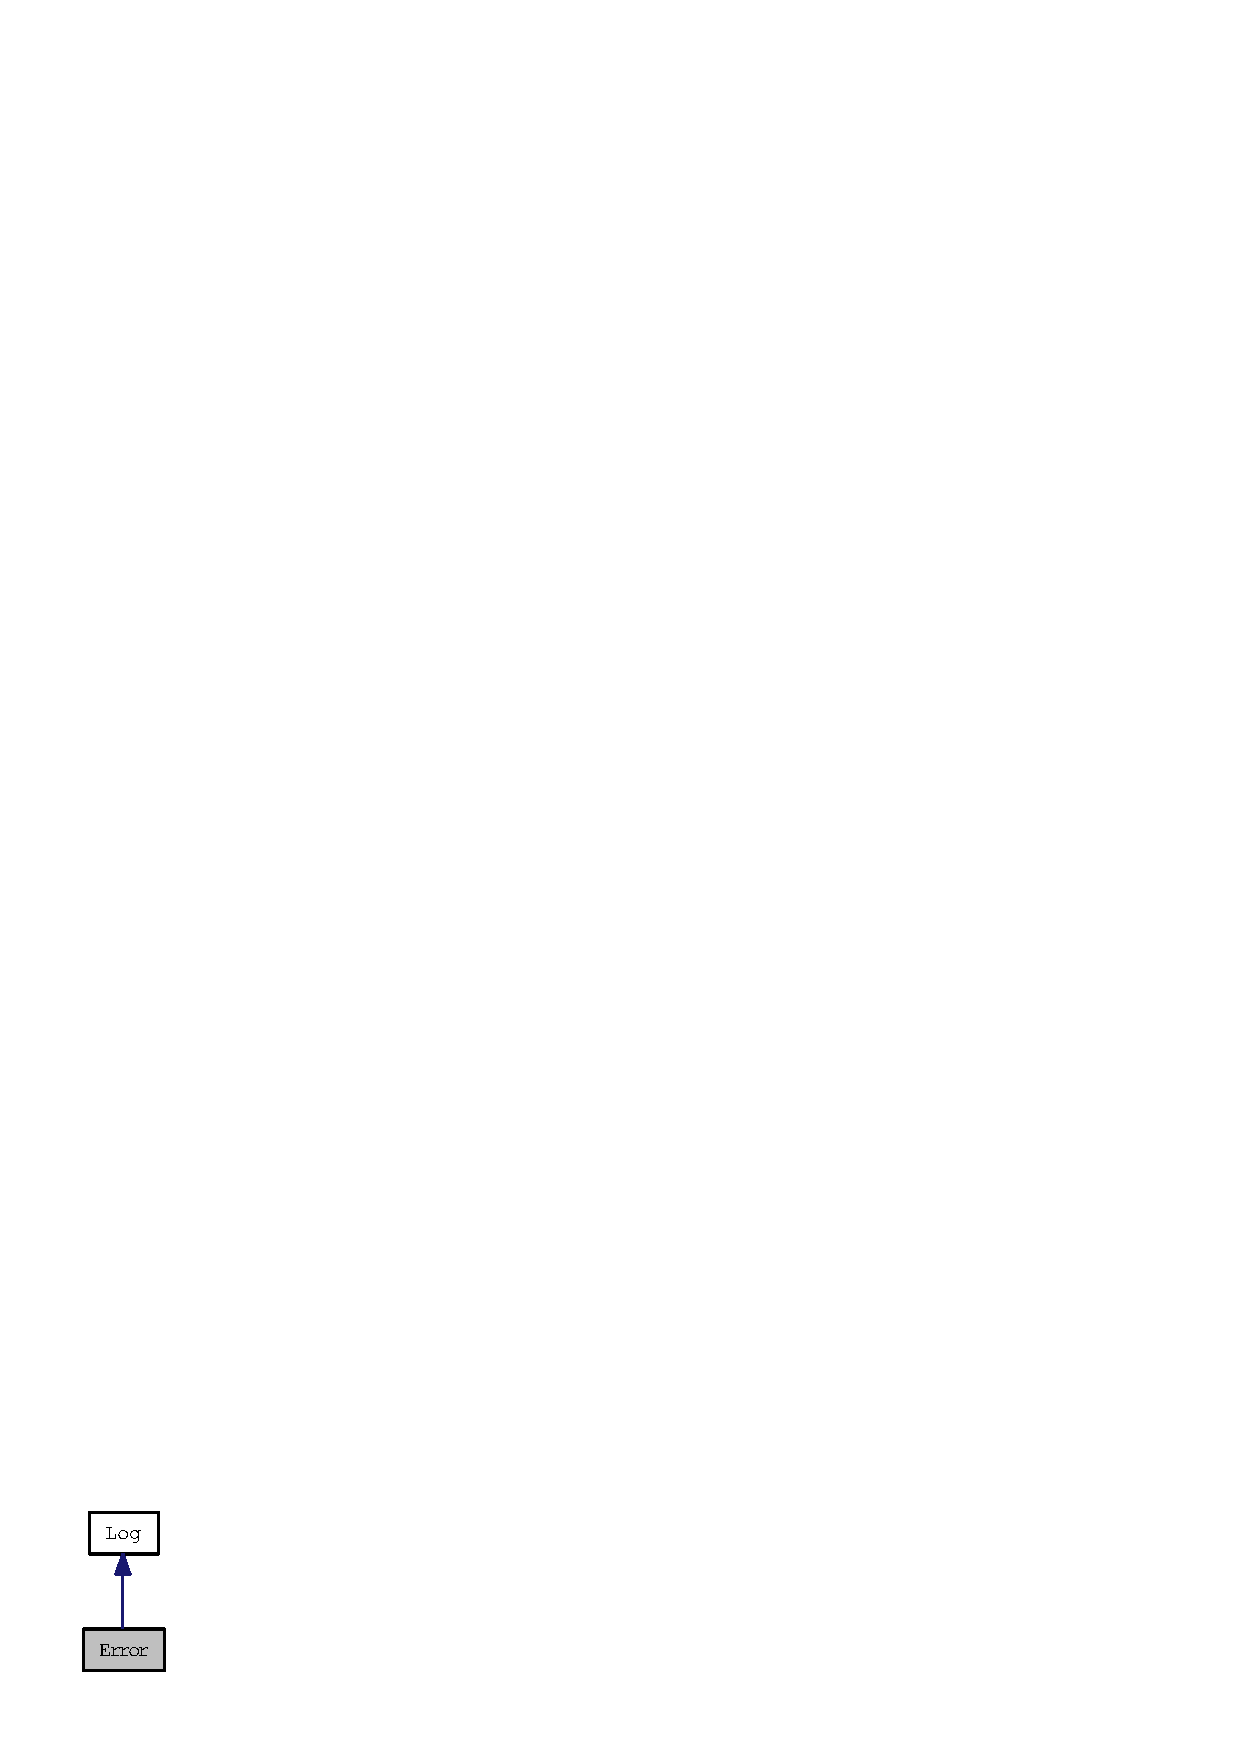
\includegraphics[width=41pt]{classError__inherit__graph}
\end{center}
\end{figure}
Collaboration diagram for Error:\nopagebreak
\begin{figure}[H]
\begin{center}
\leavevmode
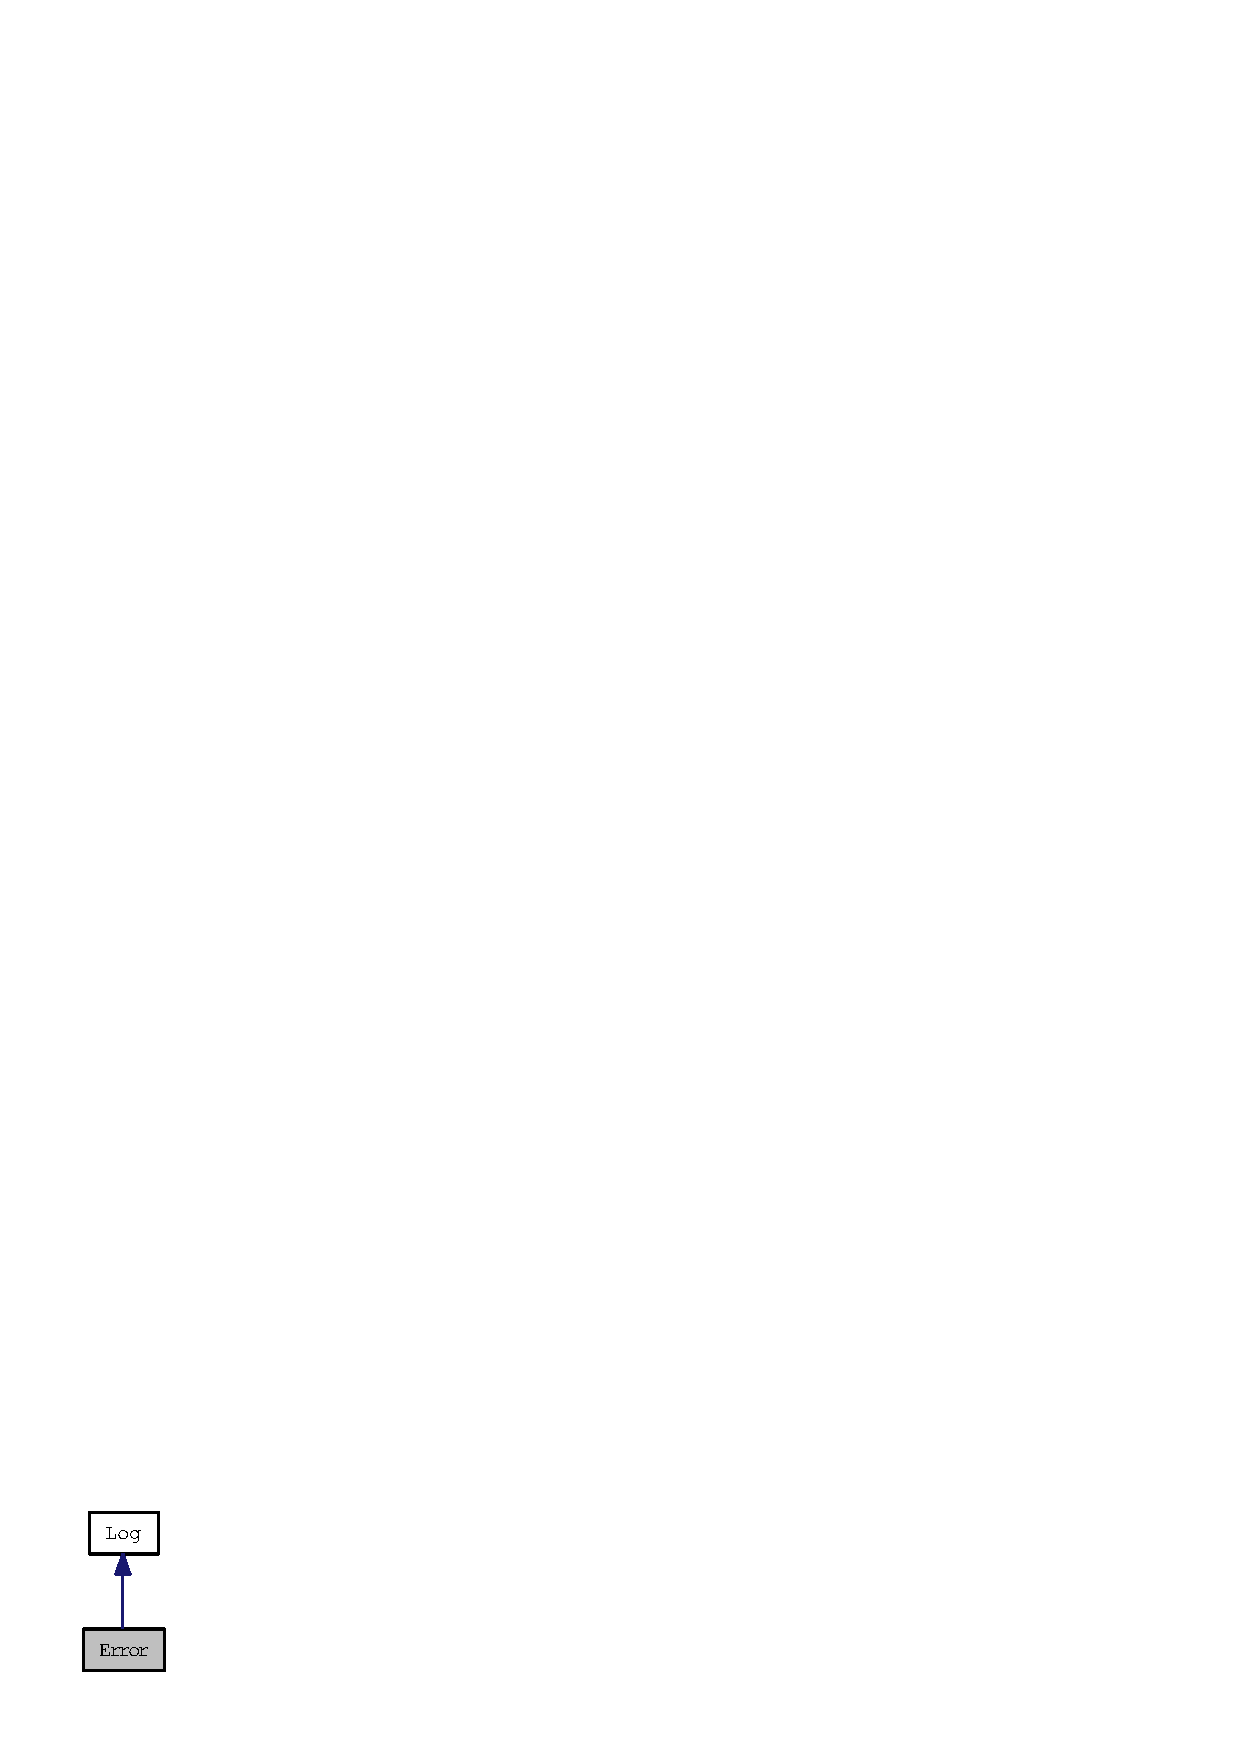
\includegraphics[width=41pt]{classError__coll__graph}
\end{center}
\end{figure}


\subsection{Detailed Description}
Stream-like class to print an error message to the app's console window Example:. 



\begin{Code}\begin{verbatim}        Error() << "This is an ERROR message!!"; // would print an error message to the console window
\end{verbatim}
\end{Code}

 

Definition at line 46 of file Log.h.

The documentation for this class was generated from the following files:\begin{CompactItemize}
\item 
Log.h\item 
Log.cpp\end{CompactItemize}

\section{Log Class Reference}
\label{classLog}\index{Log@{Log}}
Super class of \doxyref{Debug}{p.}{classDebug}, \doxyref{Warning}{p.}{classWarning}, \doxyref{Error}{p.}{classError} classes.  


{\tt \#include $<$Log.h$>$}

Inheritance diagram for Log:\nopagebreak
\begin{figure}[H]
\begin{center}
\leavevmode
\includegraphics[width=109pt]{classLog__inherit__graph}
\end{center}
\end{figure}
\subsection*{Public Member Functions}
\begin{CompactItemize}
\item 
{\footnotesize template$<$class T$>$ }\\{\bf Log} \& \textbf{operator$<$$<$} (const T \&t)\label{classLog_a743fb76f8b289cbab800e4be02a4443}

\end{CompactItemize}
\subsection*{Protected Attributes}
\begin{CompactItemize}
\item 
bool \textbf{doprt}\label{classLog_2460d2790564d76b2e067a4e82bf78d6}

\item 
QColor \textbf{color}\label{classLog_58461ea6986e1166b87ef14e28f42c01}

\end{CompactItemize}


\subsection{Detailed Description}
Super class of \doxyref{Debug}{p.}{classDebug}, \doxyref{Warning}{p.}{classWarning}, \doxyref{Error}{p.}{classError} classes. 

Definition at line 12 of file Log.h.

The documentation for this class was generated from the following files:\begin{CompactItemize}
\item 
Log.h\item 
Log.cpp\end{CompactItemize}

\section{ReentrancyPreventer Struct Reference}
\label{structReentrancyPreventer}\index{ReentrancyPreventer@{ReentrancyPreventer}}
A helper class that helps prevent reentrancy into certain functions.  


\subsection*{Public Member Functions}
\begin{CompactItemize}
\item 
{\bf ReentrancyPreventer} ()
\item 
{\bf $\sim$ReentrancyPreventer} ()
\item 
{\bf operator bool} () const \label{structReentrancyPreventer_2f9b7344c32f4096b5f73211fb5d3938}

\begin{CompactList}\small\item\em Returns true if the global counter is 1 (that is, only one globally active instance of this class exists throughout the application), and false otherwise. If false is returned, you can then abort your function early as a reentrancy condition has been detected. \item\end{CompactList}\end{CompactItemize}
\subsection*{Static Public Attributes}
\begin{CompactItemize}
\item 
static volatile int \textbf{ct} = 0\label{structReentrancyPreventer_b81c1eb29d2181821f7aec842c065303}

\end{CompactItemize}


\subsection{Detailed Description}
A helper class that helps prevent reentrancy into certain functions. 

Mainly EmulApp::loadStim(), EmulApp::unloadStim(), and EmulApp::pickOutputDir() make use of this class to prevent recursive calls into themselves.

Functions that want to be mutually exclusive with respect to each other and non-reentrant with respect to themselves need merely construct an instance of this class as a local variable, and then reentrancy into the function can be guarded by checking against this class's operator bool() function. 

Definition at line 561 of file EmulApp.cpp.

\subsection{Constructor \& Destructor Documentation}
\index{ReentrancyPreventer@{ReentrancyPreventer}!ReentrancyPreventer@{ReentrancyPreventer}}
\index{ReentrancyPreventer@{ReentrancyPreventer}!ReentrancyPreventer@{ReentrancyPreventer}}
\subsubsection{\setlength{\rightskip}{0pt plus 5cm}ReentrancyPreventer::ReentrancyPreventer ()\hspace{0.3cm}{\tt  [inline]}}\label{structReentrancyPreventer_7f5d7b40387ab9edf6575602b2121310}


Increments a global counter. The global counter is 1 if only 1 instance of this class exists throughout the application, and $>$1 otherwise. 

Definition at line 566 of file EmulApp.cpp.\index{ReentrancyPreventer@{ReentrancyPreventer}!$\sim$ReentrancyPreventer@{$\sim$ReentrancyPreventer}}
\index{$\sim$ReentrancyPreventer@{$\sim$ReentrancyPreventer}!ReentrancyPreventer@{ReentrancyPreventer}}
\subsubsection{\setlength{\rightskip}{0pt plus 5cm}ReentrancyPreventer::$\sim$ReentrancyPreventer ()\hspace{0.3cm}{\tt  [inline]}}\label{structReentrancyPreventer_83ee912ed2df8e2d8ff6d8bd656b79a9}


Decrements the global counter. If it reaches 0 this was the last instance of this class and there are no other ones active globally. 

Definition at line 569 of file EmulApp.cpp.

The documentation for this struct was generated from the following file:\begin{CompactItemize}
\item 
EmulApp.cpp\end{CompactItemize}

\section{SoundPlayer Class Reference}
\label{classSoundPlayer}\index{SoundPlayer@{SoundPlayer}}
{\tt \#include $<$SoundPlayer.h$>$}

\subsection*{Public Member Functions}
\begin{CompactItemize}
\item 
\textbf{SoundPlayer} (const QString \&filename, QObject $\ast$parent=0, bool loops=false)\label{classSoundPlayer_52bb3dd37bb3af6b78d42ede27ccd9a6}

\item 
QString \textbf{fileName} () const \label{classSoundPlayer_09a11aa0c28e1ec749cb55ae1981a161}

\item 
bool \textbf{loops} () const \label{classSoundPlayer_3e938ca6d719d32a58fae3f2081bef09}

\item 
void \textbf{play} ()\label{classSoundPlayer_15133f4990b8f8375edd0f0e6a8aa25a}

\item 
void \textbf{stop} ()\label{classSoundPlayer_11d2fd57fbb9b0b386451733f9cca5f2}

\end{CompactItemize}
\subsection*{Classes}
\begin{CompactItemize}
\item 
struct \textbf{Impl}
\end{CompactItemize}


\subsection{Detailed Description}
Abstracts out the soundplayer since on OSX we use Phonon and on all other platforms we use QSound. 

Definition at line 8 of file SoundPlayer.h.

The documentation for this class was generated from the following files:\begin{CompactItemize}
\item 
SoundPlayer.h\item 
SoundPlayer.cpp\end{CompactItemize}

\section{Status Class Reference}
\label{classStatus}\index{Status@{Status}}
Stream-like class to print a message to the app's status bar.  


{\tt \#include $<$Log.h$>$}

\subsection*{Public Member Functions}
\begin{CompactItemize}
\item 
\textbf{Status} (int timeout=0)\label{classStatus_f114ca63223e3d1d64fddeb2b7e69bb5}

\item 
{\footnotesize template$<$class T$>$ }\\{\bf Status} \& \textbf{operator$<$$<$} (const T \&t)\label{classStatus_80804dfa821ca5f0abd1ff23eaf896ca}

\end{CompactItemize}


\subsection{Detailed Description}
Stream-like class to print a message to the app's status bar. 

Definition at line 66 of file Log.h.

The documentation for this class was generated from the following files:\begin{CompactItemize}
\item 
Log.h\item 
Log.cpp\end{CompactItemize}

\section{Warning Class Reference}
\label{classWarning}\index{Warning@{Warning}}
Stream-like class to print a warning message to the app's console window.  


{\tt \#include $<$Log.h$>$}

Inheritance diagram for Warning:\nopagebreak
\begin{figure}[H]
\begin{center}
\leavevmode
\includegraphics[width=49pt]{classWarning__inherit__graph}
\end{center}
\end{figure}
Collaboration diagram for Warning:\nopagebreak
\begin{figure}[H]
\begin{center}
\leavevmode
\includegraphics[width=49pt]{classWarning__coll__graph}
\end{center}
\end{figure}


\subsection{Detailed Description}
Stream-like class to print a warning message to the app's console window. 

Example: 

\begin{Code}\begin{verbatim}        Warning() << "This is a warning message..."; // would print a warning message to the console window
\end{verbatim}
\end{Code}

 

Definition at line 59 of file Log.h.

The documentation for this class was generated from the following files:\begin{CompactItemize}
\item 
Log.h\item 
Log.cpp\end{CompactItemize}

\printindex
\end{document}
